\chapter{Background} \label{chap:background}
In order to conduct the comparison effectively, it is necessary to first lay a good theoretical basis of event-driven architecture, event stream processing and the concrete roles of an \acrshort{esp} platform. Based on that, a comprehensive set of evaluation metrics can be determined.


\section{Event Driven Architecture}
%\subsection{Monolithic Architecture}
%A monolithic application focuses on the simplicity. All components including user interface, business logic and data accessing services are developed, packaged and deployed in a single unit \cite{monolith}.

%Monolithic applications are straightforward to develop and test since the control flow is very transparent. Deployment and scaling are also simple because there is only a single software artifact. A monolithic architecture can also result in better performance for small application with few users \cite{al2018comparative}. Therefore, when starting a new software project, monolith should be the first choice to be considered \cite{monolithfirst}. 

\subsection{Microservices with Event-Driven Approach} \label{section:eventdriven}
%As the application expands, monolithic architecture gradually becomes more rigid and harder to adapt to the agile development cycle. A small change in any service will lead to rebuilding and redeployment of the entire application. Moreover, developers in the team must work closely together and cannot freely establish their own paces. For that reason, the microservices architecture arises. In general, an application is disassembled into services according to different business capabilities \cite{microservicesfowler}. These services are self-contained and loosely-coupled with each other. Each of them maintains a separate database and expose its data with other only via a mutually agreed contract. Since every service itself is an independent deployable, it can have its own development cycle and technology stack. Services also allow finer-grained scaling of the application. This is very useful for reducing cost when deploying the application to the cloud \cite{villamizar2016infrastructure}.

With microservices architecture, an application is disassembled into services according to different business capabilities \cite{microservicesfowler}. These services are self-contained and loosely-coupled with each other. Each of them maintains a separate database and expose its data with other only via a mutually agreed contract. Since every service itself is an independent deployable, it can have its own development cycle and technology stack. Services also allow finer-grained scaling of the application. This is very useful for reducing cost when deploying the application to the cloud \cite{villamizar2016infrastructure}.

In microservices architecture, services need to have a mechanism to coordinate and work together to achieve end results. There are typically two approaches for this task, namely, request-driven and event-driven \cite{stopford2018designingeventdriven}.

In the first approach, a service sends command to request for state change or queries current state in other services. This method is hard to scale because the control logic concentrates on the sender of requests. Adding a new service usually involves code change in others to include it in the control flow. For the latter approach, services communicate with each other using events.

\textbf{Event}\\
An event represents something occurred in the past and cannot be altered or deleted \cite{cqrsgregyoung}. It is simply a fact stating what has happened in the system. Whenever a service updates its state, it sends out an event. Any other service can listen and operate on this event without the sender knowing about it. This leads to inversion of control when the receiver of events now dictates the operational logic. As a result, services of the system can be more loosely coupled. New service can be easily plugged in the system and start to consume events while other services remain unmodified. There are three common ways to use events, namely, event notification, event-carried state transfer and event sourcing \cite{martinfowlereventdriven}.

\textbf{Event Notification}\\
The events are used only for notifying about a state change on the sender. Receiver decides which operation should be executed upon receiving the events. This usually involves querying for more information from either the publisher of events or another service.   
\begin{figure}[h]
	\centering
	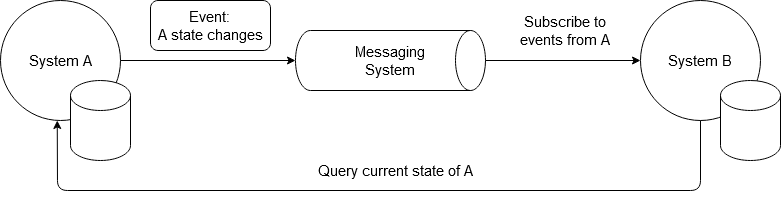
\includegraphics[width=10cm,height=5cm]{images/eventnotification.png}
	\caption{Services coordination with event notification.}
	\label{fig:eventnotification}
\end{figure}

%The approaches of event notification and request-driven ensure a minimum level of coupling by letting each service manage its own data and only share when being requested. Another advantage is that the state of each service is consistent throughout the entire system since it only exists in one place. Nevertheless, these approaches only works at their best when services are truly independent from each other which is usually not the case in reality. It is unavoidable that services must maintain a certain level of dependency and sharing of data. When services grow with more functionalities, they need to expand the service contract to expose more data to outside which then leads to higher coupling. This is known as the dichotomy of data and services \cite{stopford2018designing}. Therefore, the two following patterns tackle this problem by proactively allowing services to openly share their data instead of encapsulating it within each service.
The approaches of event notification and request-driven ensure a minimum level of coupling by letting each service manage its own data and only share when being requested. Another advantage is that the state of each service is consistent throughout the entire system since it only exists in one place. Nevertheless,when services grow with more functionalities, they need to expand the service contract to expose more data to outside which then leads to higher coupling. This is known as the dichotomy of data and services \cite{stopford2018designing}. Therefore, the two following patterns tackle this problem by proactively allowing services to openly share their data instead of encapsulating it within each service.

\textbf{Event-Carried State Transfer}\\
With this pattern, each event encloses more detail information about what has been changed as well as how it has been modified. As a result, current state of any service can be reconstructed anywhere by applying its published events on the same initial state in the same order. Therefore, every subscriber can retain a local state replica and keep it synchronized with the source of events.

\begin{figure}[h]
	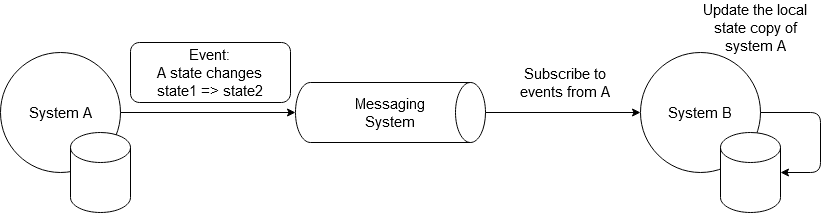
\includegraphics[width=\linewidth]{images/eventstatetransfer.png}
	\caption{Services coordination with event-carried state transfer.}
	\label{fig:eventstatetransfer}
\end{figure}

When a service keeps a state copy of another locally, it can access this data faster and becomes independent of the online status of the source of data. Nevertheless, having multiple copies of data across the system also means that the system can be in inconsistent state temporarily or even worse permanently if it is not designed carefully. This concern is closely related to the problem of how to atomically update the local state and publish a corresponding event \cite{eventstatetransferproblem}.

%\textbf{Event Sourcing and \acrfull{cqrs}}\\
\textbf{Event Sourcing}\\
The event sourcing pattern takes one step further. Events are not used to only notify and help replicate states among services but they are now the primitive form of data store \cite{eventsourcingfowler}. Instead of updating the current state, services record every state change as events which are stored in the order of occurring in append-only fashion. This stream of events becomes the source of truth for the entire system. Services can derive the state of any entity from the events stream and keep it in memory or a cache to query when needed. Snapshot of the current state can be periodically created to avoid processing through all events after every restart.

\begin{figure}[h]
	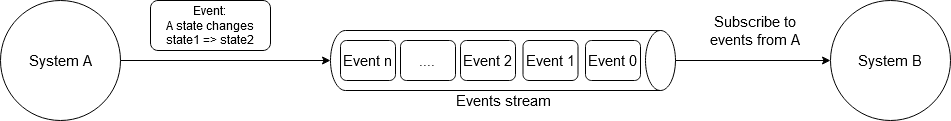
\includegraphics[width=\linewidth]{images/eventsourcing.png}
	\caption{Services coordination with event sourcing.}
	\label{fig:eventsourcing}
\end{figure}

This approach eliminates the need of atomically updating state and generating event as in event-carried state transfer since there is now only publishing of events. Apart from providing a loosely-coupled and scalable way for coordination among services, event sourcing comes with additional benefits. The stream of events retains the entire history of the system and therefore can be used for auditing, extracting more value from past events, troubleshooting problem during production as well as for testing and fixing errors by simply replaying the events with the new system \cite{betts2013exploring}. 

%Event sourcing is often used together with CQRS \cite{cqrsgregyoung}. The CQRS pattern promotes the idea of having two independent sides of command and query corresponding to two separate models for writing and reading data respectively. By doing this, each model can scale independently based on the load of each side. Moreover, this gives the flexibility to derive multiple ways to query data on the reading side without being tightly coupled to the data model of the input side. 

%\begin{figure}[h]
%	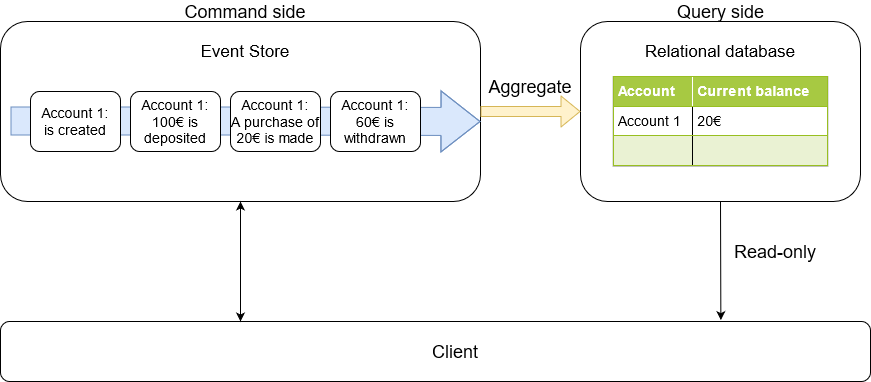
\includegraphics[width=\linewidth]{images/cqrs.png}
%	\caption{Event sourcing and CQRS.}
%	\label{fig:cqrs}
%\end{figure}

%In the context of event sourcing, the command side of CQRS is the stream of events. Greg Young pointed out a number of reasons why this is a good writing model \cite{cqrsgregyoung}. The append-only operation to add new events makes it more scalable. Moreover, there is no impedance mismatch between domain model of the application and the storage model as in the case of relational database because event is also a domain concept. On the query side, the representation of current state are created with the underline events stream. Figure \ref{fig:cqrs} illustrates an example of a simple bank account management system. Transactions of users are recorded as events. The queryable current account balance is derived by aggregating the history of transactions and writing it to a relational database which is solely for reading.

Event-driven architecture and its related patterns are useful but it also comes with a cost of increasing complexity in the system \cite{eventsourcingishard1} \cite{eventsourcingishard2}. As can be seen from the above short summary, one of the most significant added values of this approach is to reduce the coupling and lay the foundation for systems with high demand for scalability. If this is not the case, a simpler approach should be chosen to not overcomplicate the system.




\section{Stream Processing} \label{section:eventstreamprocessing}
With the increasing amount of data, the demand about how data is processed and analyzed also evolves over time. With the batch processing paradigm, data is collected over a predefined period of time and stored in a big bounded batch in a data warehouse. Some scheduled batch jobs will then go over the entire batch of data to generate insights and reports tying to the needs of organizations. However, this type of data processing gradually cannot keep up with the need of faster analysis to allow companies to response more timely to changes. Therefore, the concept of stream processing begins to emerge.


Unlike its batch counterpart, stream processing aims at handling unbounded data which is a better form for representing the flow of events in real world given their continuous and boundless nature. Stream processing frameworks are designed to handle this type of data with high throughput and horizontal scalability. A stream processor can ingest one or more input streams and execute its business logic. It can also generate new data to other output streams which subsequently can be consumed by other stream processors. The data flow is continuous and new stream processors can always be added to incorporate new processing logic and generate more results.

\begin{figure}[h]
	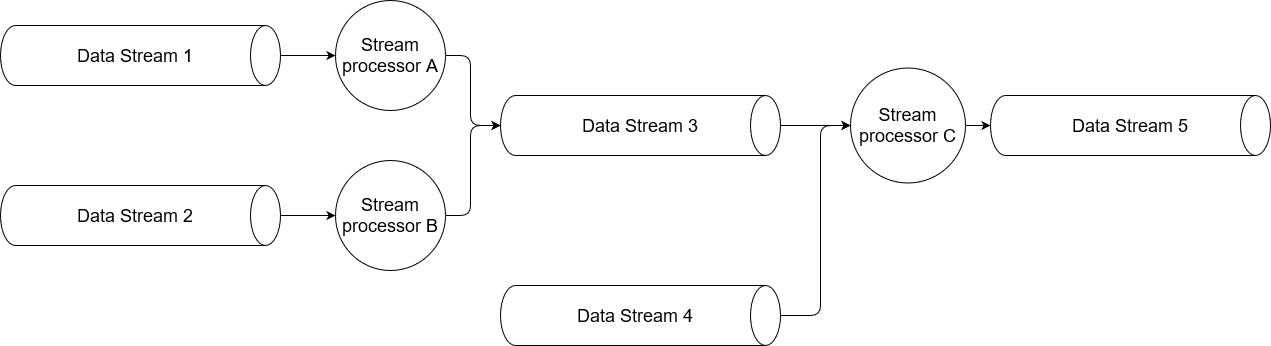
\includegraphics[width=\linewidth]{images/streamprocessing.png}
	\caption{Stream processing concept.}
	\label{fig:streamprocessing}
\end{figure}


By processing this influx of data continuously as they arrives, events and patterns can be detected with low latency making stream processing more suitable for real-time use cases. Moreover, the input data can come from numerous sources with varying transmission rates. Therefore, data may arrive late and out of order with respect to the time it is generated at the source. In this case, for it sees data in an endless fashion, stream processing gives more tolerance for late data and more flexibility to assemble data into windows and sessions to extract more useful information. It is even suggested that a well-designed stream processing system with guarantee of correctness and the capability to effectively manage the time semantics could surpass batch processing system \cite{stream101}. Back in the time when using stream processing was a trade-off between accuracy and low-latency, it was a popular idea to run two batch and stream processing pipelines in parallel to achieve both fast and correct results \cite{lambdaarchitecture}.  As stream processing engines grow more mature and accurate, the demand for such system is lessened \cite{questionlambdaarchitecture}.
\subsection{Stream Processing and Event-Driven Architecture}

Stream processing is not merely a data processing paradigm to achieve low latency result. Applying the concept of streaming and event-driven architecture on the organizational level also has the potential to help build more scalable and resilient software infrastructure for organizations. A big institution using software in every operational aspect usually has a sophisticated software infrastructure providing different functionalities such as business applications, query and analytical services, monitoring system, data warehouse. In this case, the problem of coupling emerges not only between services of applications but also between these processing and data systems on a bigger scale. Data needs to be shared and synchronized between these components. Without an efficient way to integrate system-wide data, the entire system can quickly turns into a big tangled mesh. As an example, this problem was experienced at LinkedIn as their system became increasingly complex \cite{eventstreamingplatform}. 

\begin{figure}[h]
	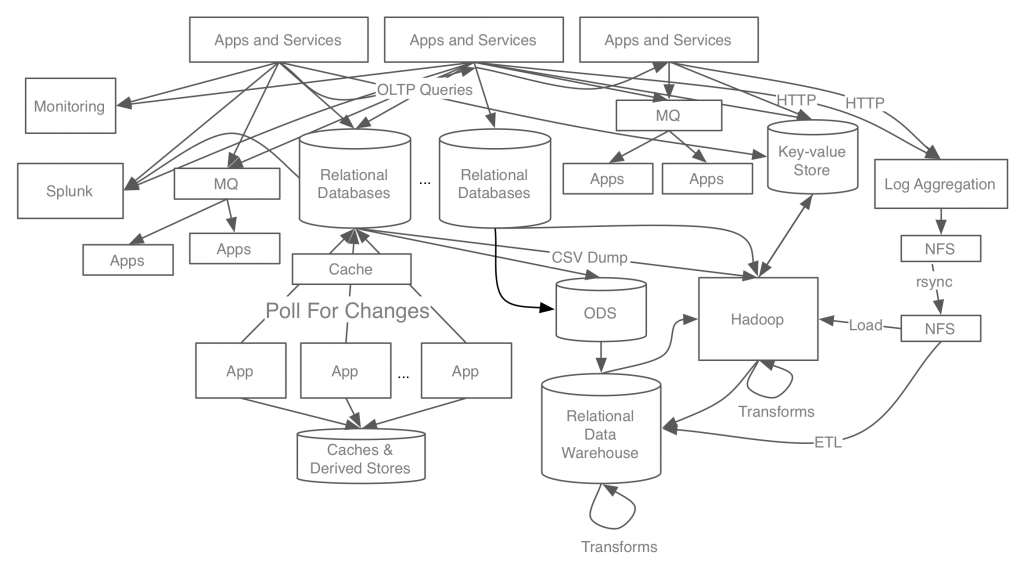
\includegraphics[width=\linewidth,height=7.5cm]{images/linkedin-data-flow-ugly.png}
	\caption{The tangled data systems at LinkedIn in the old day \cite{eventstreamingplatform}.}
	\label{fig:tangledsystem}
\end{figure}

Jay Kreps described in his article a log-centric infrastructure that can solve this problem \cite{logjaykreps}. Every event recorded by any data system in the organization, is written orderly to an append-only log. This becomes the backbone for all data systems in the organization similar to using event-sourcing in a distributed system but on a much bigger scale. Each system has the flexibility to derive different data structures from the raw events to match its specific access pattern. The task of data representation is now done at individual system instead of in the central data store. 
%This is referred by Martin Kleppmann as turning the database inside out \cite{kleppmann2016making}. With this approach, an entire software infrastructure of organization now turns into a gigantic distributed database with the log of events lying at the center and all systems are simply indexes on the raw data in the form of events \cite{logjaykreps}. 



Processing streams of events on an organizational scale is a non-trivial task. This is where stream processing fits in by providing a scalable tool to handle such amount of data. Applications and their decoupled services can use stream processing to continuously consume, process and generate new events while data systems can use streaming tool to continuously integrate new data from the streams to their data representation. The result is a more neatly organized infrastructure with every system synchronizes and communicates via the event streams using stream processing. 

\begin{figure}[h]
	\centering
	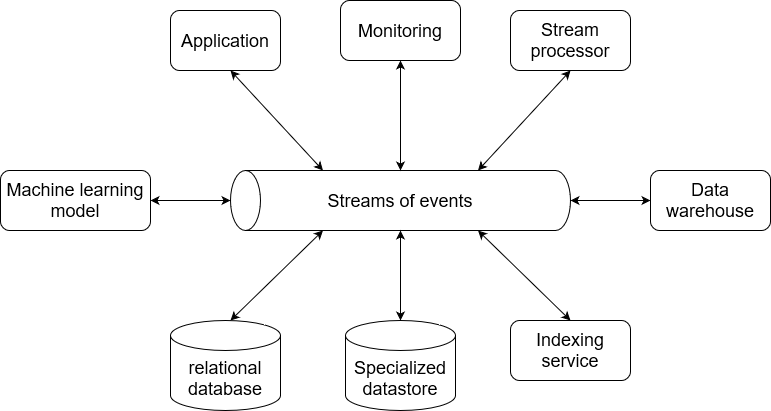
\includegraphics[width=10cm,height=5cm]{images/eventstreamprocessing.png}
	\caption{System with streams of events as the single source of truth.}
	\label{fig:eventstreamprocessingsystem}
\end{figure}

%Any data service in the system can consume and process this log of raw events using stream processing to generate a local replication of the current system state. This log-centric design fits seamlessly into a distributed environment with numerous moving components to allow data to be replicated among services with minimal coupling \cite{logjaykreps}. 



\section{\acrlong{esp} Platform} \label{section:general-ESP-platform}
An \acrshort{esp} platform must facilitate the construction of software systems revolving around streams of events. According to Jay Kreps, it has two main uses \cite{eventstreamingplatform}. Firstly, it must provide the necessary infrastructure and tools for applications to work and coordinate with each other on top of events streams. Secondly, the platform can serve as the integration point where various data systems can attach themselves into and synchronize data among them continuously.

To fulfill these two uses, the following fundamental capabilities are required. A platform must have an events storage layer. Optimally, it should also support the option to persist events for an infinite period of time since this will be the single source of truth that all data systems depend on. Accessing interface must be provided for applications to publish and consume events. Based on this, custom applications and services can already be self-implemented to do stream processing as well as integrating data to different destinations. However, such platform only provides minimal functionalities and burdens developers with many low-level implementation tasks.

In order to be more useful and easier to be integrate into the infrastructure of organizations, an \acrshort{esp} platform must provide more supporting tools. More particularly, the platform should also support the processing of events streams either by providing a native stream processing tool or being able to integrate with external stream processing framework. For the data integration, the platform should come with ready-to-be-used tools to integrate with a wide range of existing data systems effortlessly including also legacy systems. Moreover,the platform should have a rich set of utility tools for monitoring and management.

\begin{figure}[h]
	\centering
	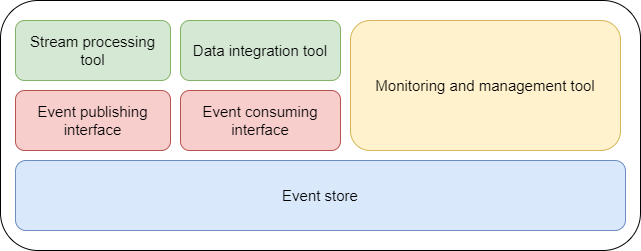
\includegraphics[width=10cm,height=5cm]{images/espplatform.png}
	\caption{Capabilities of an \acrshort{esp} platform.}
	\label{fig:espplatform}
\end{figure}


All of these capabilities should be in a real-time, high throughput, scalable and highly reliable fashion so that the platform would not become the bottleneck in the infrastructure. 

%The order of events must be preserved by the platform throughout their entire life cycle: in storage, transit and under process. All of these capabilities should be in a real-time, high throughput, scalable and highly reliable fashion so that the platform would not become the bottleneck in the infrastructure. Finally, the platform should have a rich set of utility tools for monitoring and management.



